\documentclass[unicode,11pt,a4paper,oneside,numbers=endperiod,openany]{scrartcl}

\usepackage{ifthen}
\usepackage[utf8]{inputenc}
\usepackage{graphics}
\usepackage{graphicx}
\usepackage{hyperref}
%%%%%%%%%%%%%%%%%%%%% Added Packages: %%%%%%%%%%%%%%%%%%%%%%%%%%%%%%%%%%
\usepackage{amsmath}
\usepackage{float}

\usepackage[dvipsnames]{xcolor}
\usepackage{fancyvrb}

\usepackage{subcaption}
\usepackage{ifthen}
\usepackage{listings}



% redefine \VerbatimInput
\RecustomVerbatimCommand{\VerbatimInput}{VerbatimInput}%
{fontsize=\footnotesize,
 %
 frame=lines,  % top and bottom rule only
 framesep=2em, % separation between frame and text
 rulecolor=\color{Gray},
 %
%  label=\fbox{\color{Black}slurm-euler\_phase\_1.txt},
%  labelposition=topline,
 %
 commandchars=\|\(\), % escape character and argument delimiters for
                      % commands within the verbatim
 commentchar=*        % comment character
}

% \newcommand{\myInputFile}{slurm-euler_phase_1.txt} % Set the default input file
% \newboolean{isPhaseOne}
% \setboolean{isPhaseOne}{true} % Set to false for phase 2

% % Redefine \VerbatimInput
% \RecustomVerbatimCommand{\VerbatimInput}{VerbatimInput}%
% {
%     fontsize=\footnotesize,
%     frame=lines,  % top and bottom rule only
%     framesep=2em, % separation between frame and text
%     rulecolor=\color{Gray},
%     label=\fbox{\ifthenelse{\boolean{isPhaseOne}}{\color{Black}slurm-euler\_phase\_1.txt}{\color{Black}slurm-euler\_phase\_2.txt}},
%     labelposition=topline,
%     commandchars=\|\(\), % escape character and argument delimiters for
%                           % commands within the verbatim
%     commentchar=*        % comment character
% }
%%%%%%%%%%%%%%%%%%%%%%%%%%%%%%%%%%%%%%%%%%%%%%%%%%%%%%%%%%%%%%%%%%%%%%%

\pagestyle{plain}
\voffset -5mm
\oddsidemargin  0mm
\evensidemargin -11mm
\marginparwidth 2cm
\marginparsep 0pt
\topmargin 0mm
\headheight 0pt
\headsep 0pt
\topskip 0pt        
\textheight 255mm
\textwidth 165mm

\newcommand{\duedate} {}
\newcommand{\setduedate}[1]{%
\renewcommand\duedate {Due date:~ #1}}
\newcommand\isassignment {false}
\newcommand{\setassignment}{\renewcommand\isassignment {true}}
\newcommand{\ifassignment}[1]{\ifthenelse{\boolean{\isassignment}}{#1}{}}
\newcommand{\ifnotassignment}[1]{\ifthenelse{\boolean{\isassignment}}{}{#1}}

\newcommand{\assignmentpolicy}{
\begin{table}[h]
\begin{center}
\scalebox{0.8} {%
\begin{tabular}{|p{0.02cm}p{16cm}|}
\hline
&\\
\multicolumn{2}{|c|}{\Large\textbf{HPC Lab for CSE 2024 ---  Submission Instructions}}\\
\multicolumn{2}{|c|}{\large\textbf{(Please, notice that following instructions are mandatory: }}\\
\multicolumn{2}{|c|}{\large\textbf{submissions that don't comply with, won't be considered)}}\\
&\\
\textbullet & Assignments must be submitted to \href{https://moodle-app2.let.ethz.ch/course/view.php?id=22516}{Moodle} (i.e. in electronic format).\\
\textbullet & Provide both executable package and sources (e.g. C/C++ files, Matlab). 
If you are using libraries, please add them in the file. Sources must be organized in directories called:\\
\multicolumn{2}{|c|}{\textit{Project\_number\_lastname\_firstname}}\\
& and  the  file must be called:\\
\multicolumn{2}{|c|}{\textit{project\_number\_lastname\_firstname.zip}}\\
\multicolumn{2}{|c|}{\textit{project\_number\_lastname\_firstname.pdf}}\\
\textbullet &  The TAs will grade your project by reviewing your project write-up, and looking at the implementation 
                 you attempted, and benchmarking your code's performance.\\

\textbullet & You are allowed to discuss all questions with anyone you like; however: (i) your submission must list anyone you discussed problems with and (ii) you must write up your submission independently.\\
\hline
\end{tabular}
}
\end{center}
\end{table}
}
\newcommand{\punkte}[1]{\hspace{1ex}\emph{\mdseries\hfill(#1~\ifcase#1{Points}\or{Points}\else{Points}\fi)}}


\newcommand\serieheader[6]{
\thispagestyle{empty}%
\begin{flushleft}

\includegraphics[width=0.4\textwidth]{Images/ETHlogo_13}
\end{flushleft}
  \noindent%
  {\large\ignorespaces{\textbf{#1}}\hspace{\fill}\ignorespaces{ \textbf{#2}}}\\ \\%
  {\large\ignorespaces #3 \hspace{\fill}\ignorespaces #4}\\
  \noindent%
  \bigskip
  \hrule\par\bigskip\noindent%
  \bigskip {\ignorespaces {\Large{\textbf{#5}}}
  \hspace{\fill}\ignorespaces \large \ifthenelse{\boolean{\isassignment}}{\duedate}{#6}}
  \hrule\par\bigskip\noindent%  \linebreak
 }

\makeatletter
\def\enumerateMod{\ifnum \@enumdepth >3 \@toodeep\else
      \advance\@enumdepth \@ne
      \edef\@enumctr{enum\romannumeral\the\@enumdepth}\list
      {\csname label\@enumctr\endcsname}{\usecounter
        {\@enumctr}%%%? the following differs from "enumerate"
	\topsep0pt%
	\partopsep0pt%
	\itemsep0pt%
	\def\makelabel##1{\hss\llap{##1}}}\fi}
\let\endenumerateMod =\endlist
\makeatother




\usepackage{textcomp}






\begin{document}


\setassignment
\setduedate{25 March 2024, 23:59}

\serieheader{High-Performance Computing Lab for CSE}{2024}
            {Student: Yannick Ramic}
            {Discussed with: Carla Lopez}{Solution for Project 2}{}
\newline

\assignmentpolicy

\section{Computing $\pi$ with \texttt{OpenMP} [20 points]}
The very first exercise task, comprises of two subtasks, where the goal of this omp introductory exercise is to 
implement two versions of parallelized code. The underlying serial implementation is already given and provides 
the template on how to compute $\pi$ numerically, by approximating the integral with the midpoint rule, as explained 
in the exercise sheet. To speed up this task we should implement 2 different parallelized versions, one with the 
\textit{critical} directive and the other one with the \textit{reduction} clause. Besides the lecture notes the 
information to solve this task was taken from the introductory book by Hager and Wellein \cite{HPC}.
\newline \indent
As described in \cite{HPC}, OpenMP provides a more elegant way, compared to an implementation with a critical region, 
in order to update a variable. Thus, I will start with explaining the advantage of using the \textit{Reduction} clause.
The \textit{Reduction} clause expects a definition of the used operator, which is in our case the $+$ operator because 
we accumulate values at each iteration, by simply summing over them. Besides the operator we have to define our target 
value, which is in this case \textit{sum}. As a result, the specified variable will be privatized and initialized with 
a sensible initial value. In the end, obviously we need to synchronize each thread again. Thus, in the end all partial results 
in this case will be accumulated and stored in the variable sum. \cite{HPC}
\newline \indent
Another possibility, also described in \cite{HPC}, is to define critical regions, in order to achieve a fast parallelized 
version of a serial code implementation. Critical regions can become necessary, in order to avoid concurrent overwriting and 
sharing a variable. This problem is called race condition and can be avoided by allowing only one thread executing code in this 
defined code part. The order in which threads access this region of code is undefined but also here are possibilities if 
necessary. At this point it's important to mention that a wrong use of the \textit{critical} directive can lead to another 
problem called deadlocks, where one or more threads become inactivate and wait for resources that become never available. 
This problem typically occurs when two or more critical regions are badly arranged. For instance, when a thread encounters 
another critical directive inside a critical region, it will be blocked forever. In order to avoid this, OpenMP also provides 
the solution of naming the critical region, which offers the opportunity to distinguish each region. \cite{HPC}
\begin{figure}[H]
  \centering
  {\fontsize{8}{10}\selectfont
  \VerbatimInput{Images_Output/critical_reduction.txt}}
  \caption{Critical and Reduction Based Parallelization Version}
  \label{fig:critical_reduction}
\end{figure}
Before presenting the strong and weak scaling analysis, the underlying code for both versions can be found in 
\ref{fig:critical_reduction}. As mentioned in the last task it's necessary to benchmark the performance of each parallelized 
version. Weak scaling asks the question, how well does the prallel fraction scale among p processors? 
code. 
\newpage
\begin{figure}[H]
    \centering
    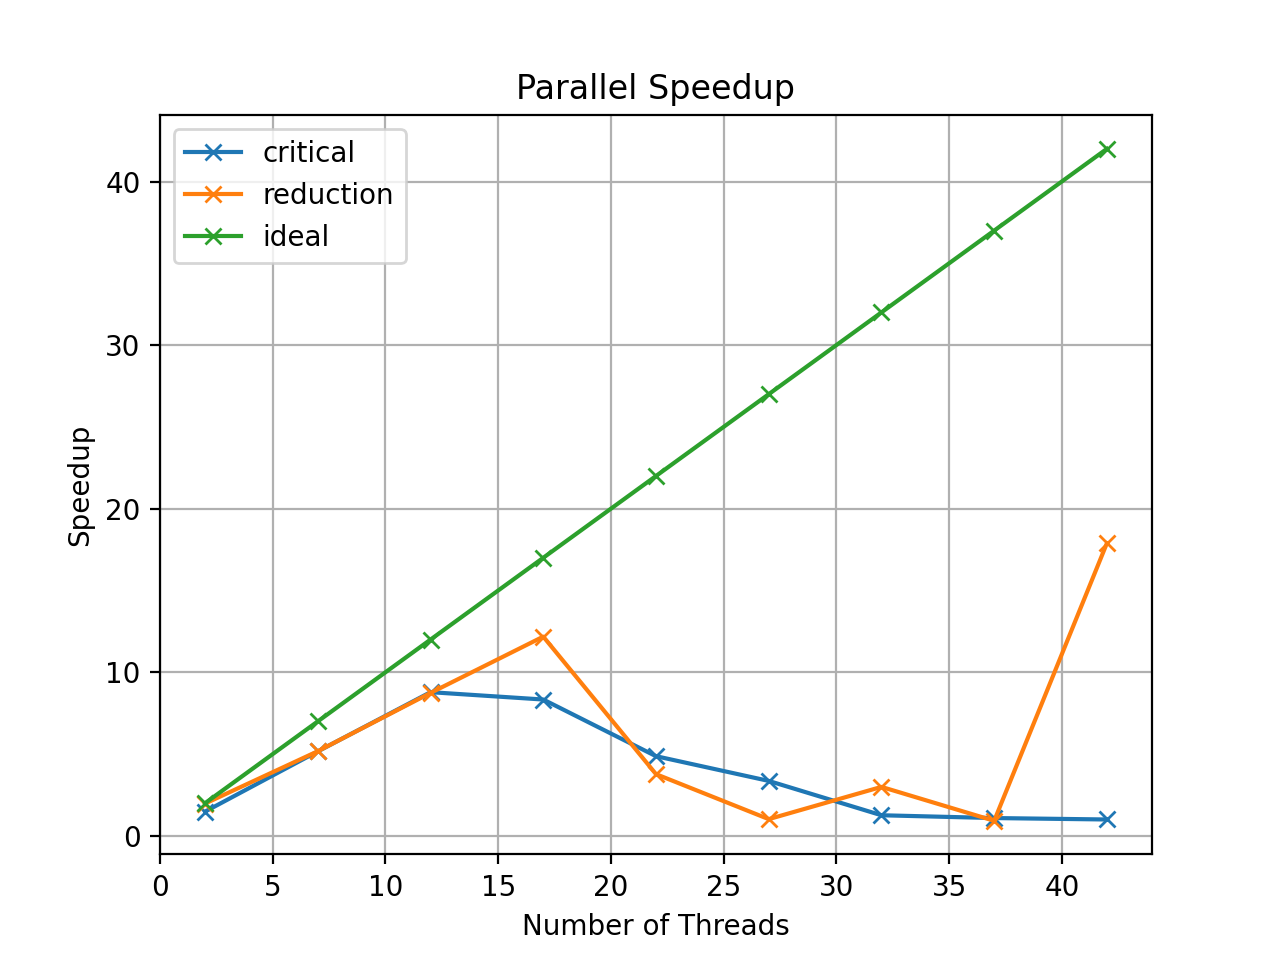
\includegraphics[width=0.9\textwidth]{Images_Output/parallel_speedup.png}
    \caption{Strong Scaling Analysis: Parallel Speedup}
    \label{fig:strong_scaling}
  \end{figure}
\begin{figure}[H]
    \centering
    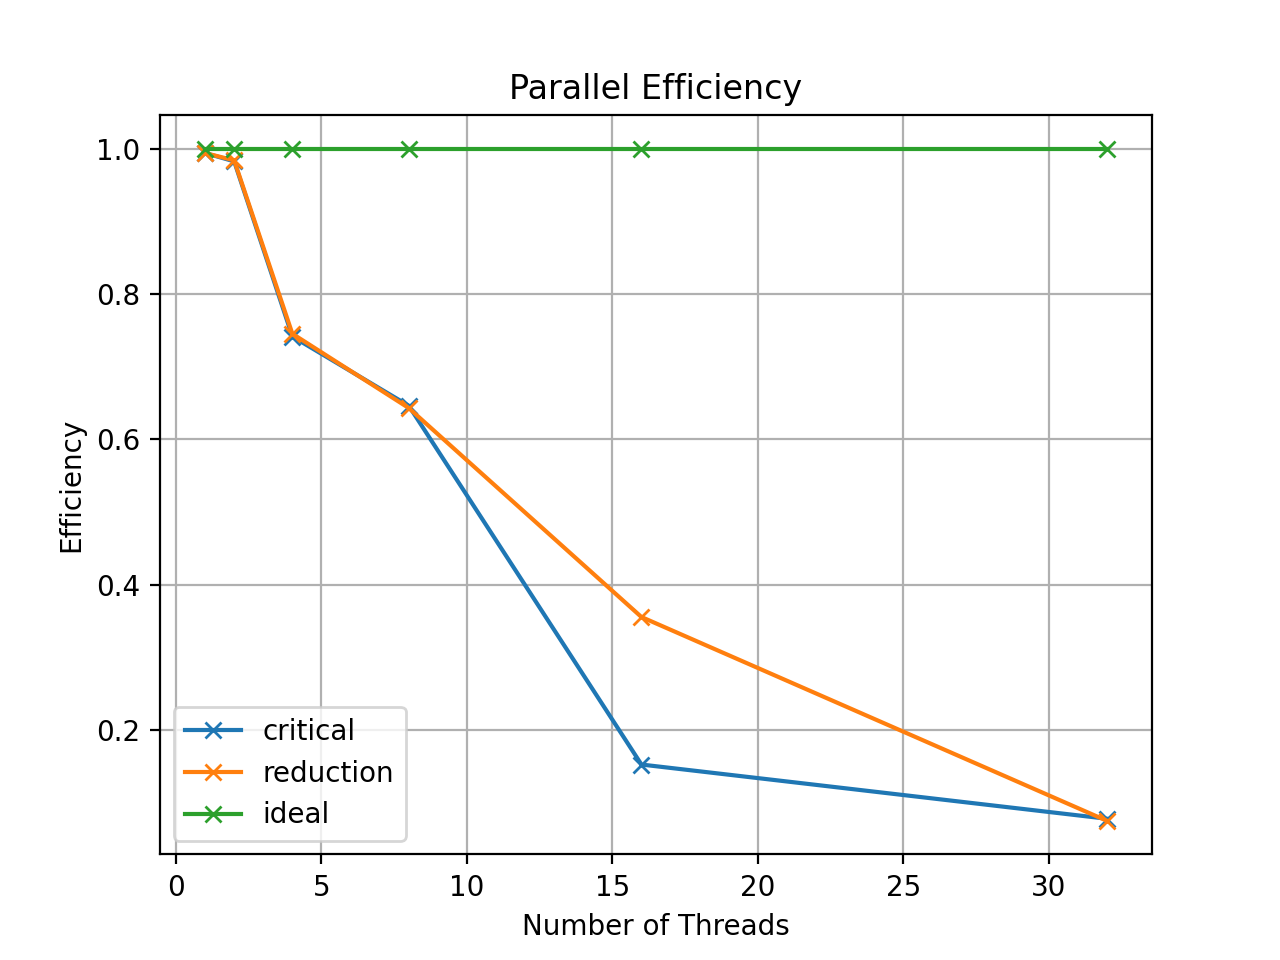
\includegraphics[width=0.9\textwidth]{Images_Output/parallel_efficiency.png}
    \caption{Weak Scaling Analysis: Parallel Efficiency}
    \label{fig:weak_scaling}
  \end{figure}

\section{The Mandelbrot set  using \texttt{OpenMP} [20 points]}

\begin{figure}[H]
  \centering
  
\includegraphics[width=0.7\textwidth]{Images_Output/mandel.png}
  \caption{Quicksort algorithm, retrived from \cite{parallelized_quicksort}}
  \label{fig:quicksort}
\end{figure}
\begin{figure}[H]
  \centering
  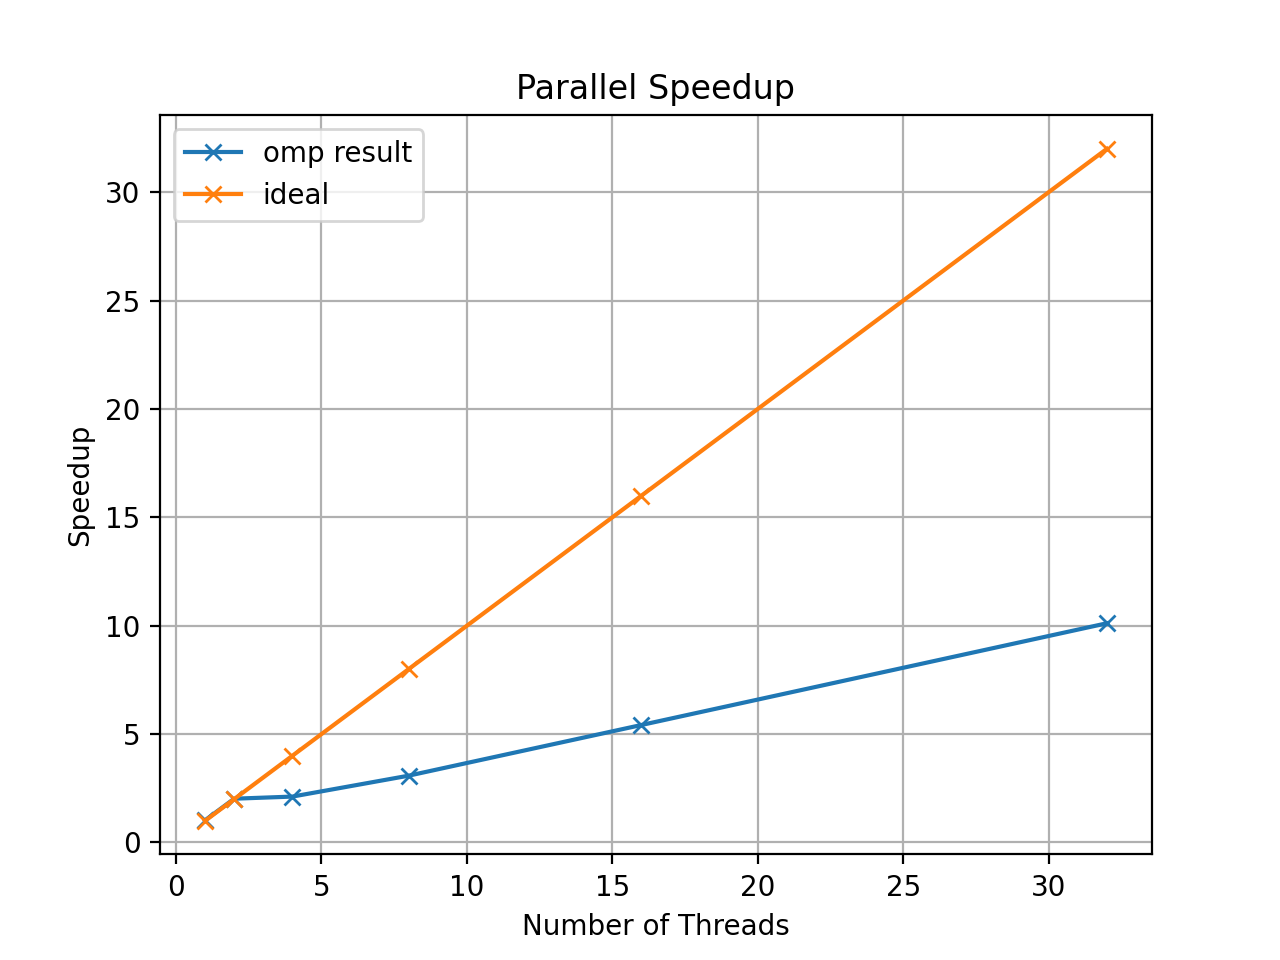
\includegraphics[width=0.8\textwidth]{Images_Output/mandel_speedup.png}
  \caption{Quicksort algorithm, retrived from \cite{parallelized_quicksort}}
  \label{fig:quicksort}
\end{figure}

\section{Bug hunt [10 points]}

\section{Parallel histogram calculation using \texttt{OpenMP} [15 points]}

\begin{figure}[H]
  \centering
  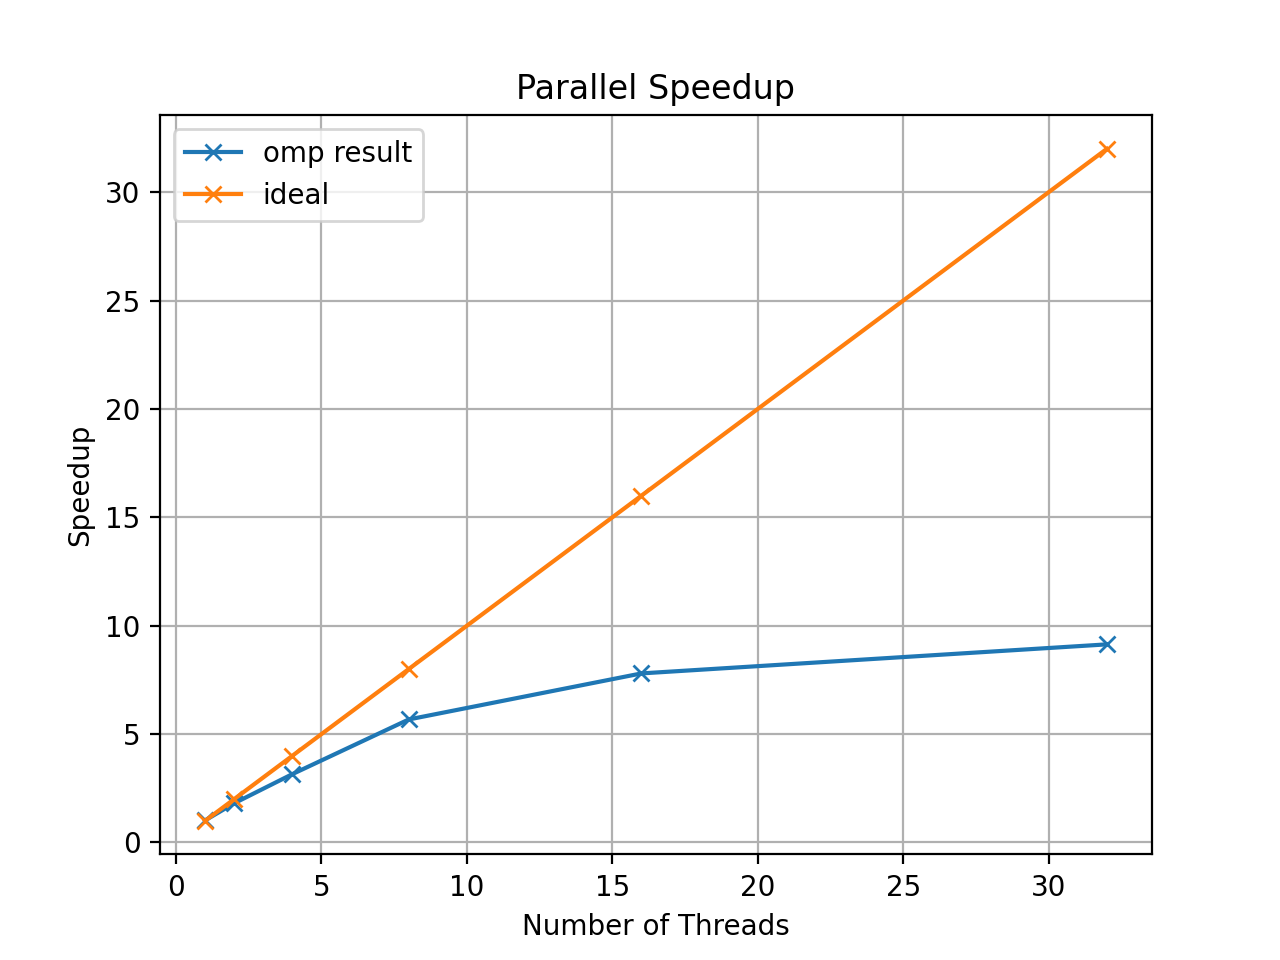
\includegraphics[width=\textwidth]{Images_Output/hist_speedup.png}
  \caption{Quicksort algorithm, retrived from \cite{parallelized_quicksort}}
  \label{fig:quicksort}
\end{figure}

\section{Parallel loop dependencies with \texttt{OpenMP} [15 points]}

\begin{figure}[H]
  \centering
  {\fontsize{8}{10}\selectfont
  \VerbatimInput{Images_Output/sequential_code_snippet.txt}}
  \caption{Loop Dependencies Problem Description}
  \label{fig:slurm_euler_2}
\end{figure}

\begin{figure}[H]
  \centering
  {\fontsize{8}{10}\selectfont
  \VerbatimInput{Images_Output/parallelized_code_snippet.txt}}
  \caption{Parallelized Code Snippet}
  \label{fig:slurm_euler_2}
\end{figure}

\section{Quicksort using \texttt{OpenMP} tasks [20 points]}

\begin{figure}[H]
  \centering
  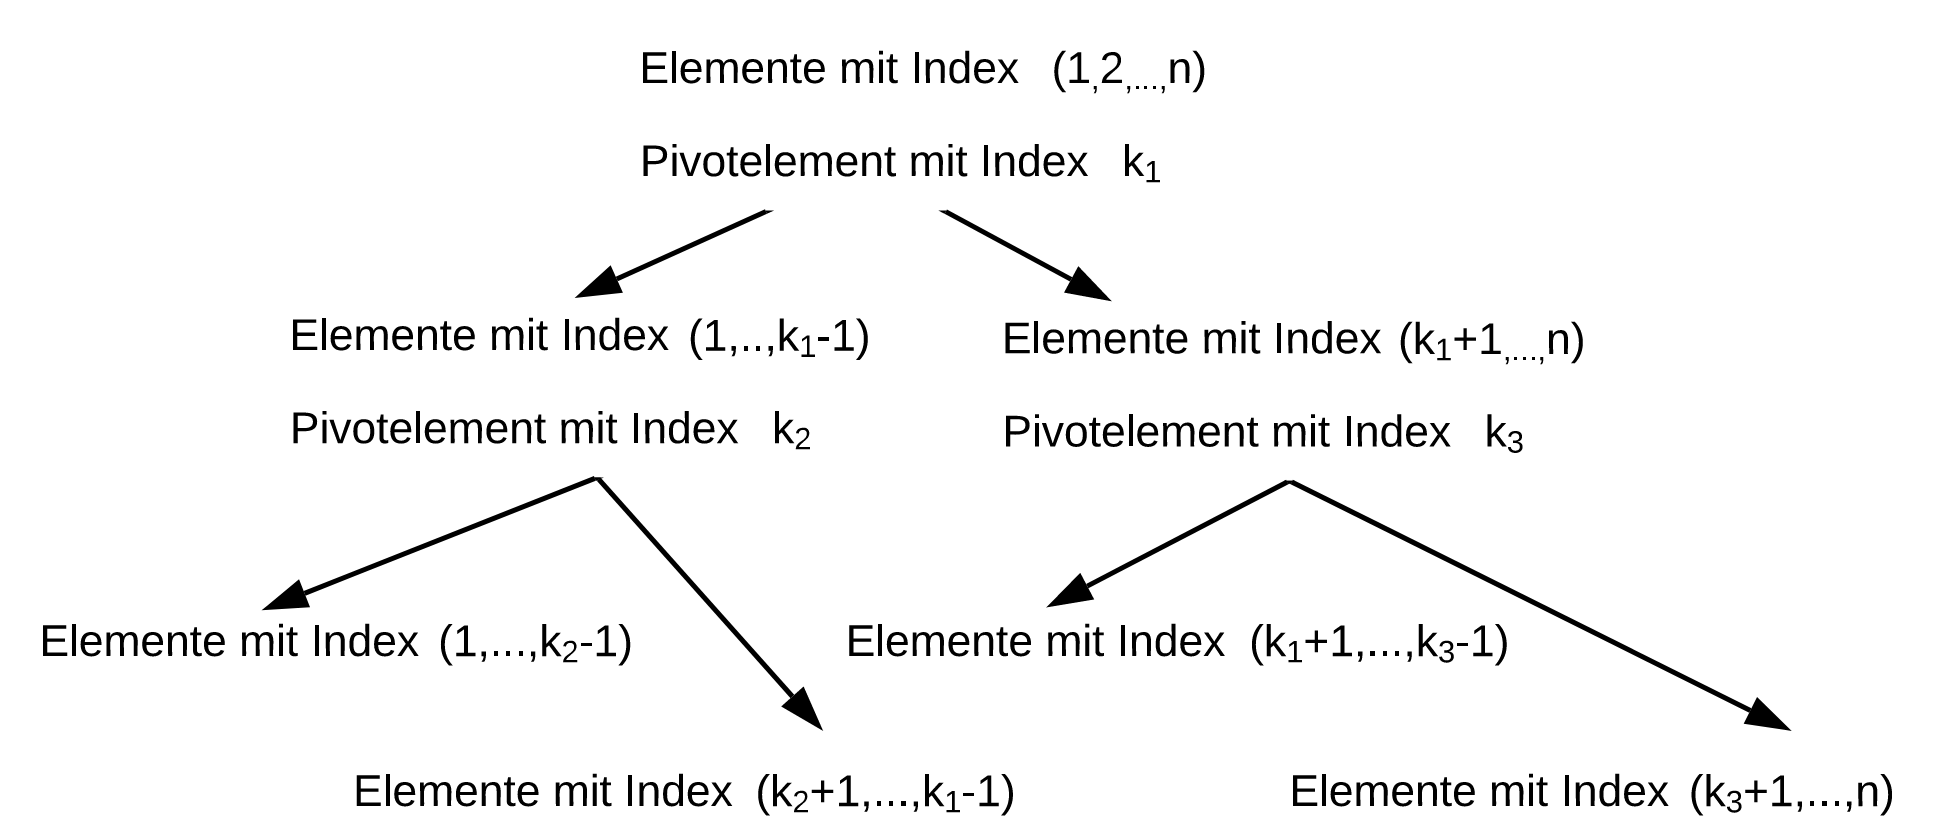
\includegraphics[width=\textwidth]{Images_Output/Quicksort.png}
  \caption{Quicksort algorithm, retrived from \cite{parallelized_quicksort}}
  \label{fig:quicksort}
\end{figure}

\begin{figure}[H]
  \centering
  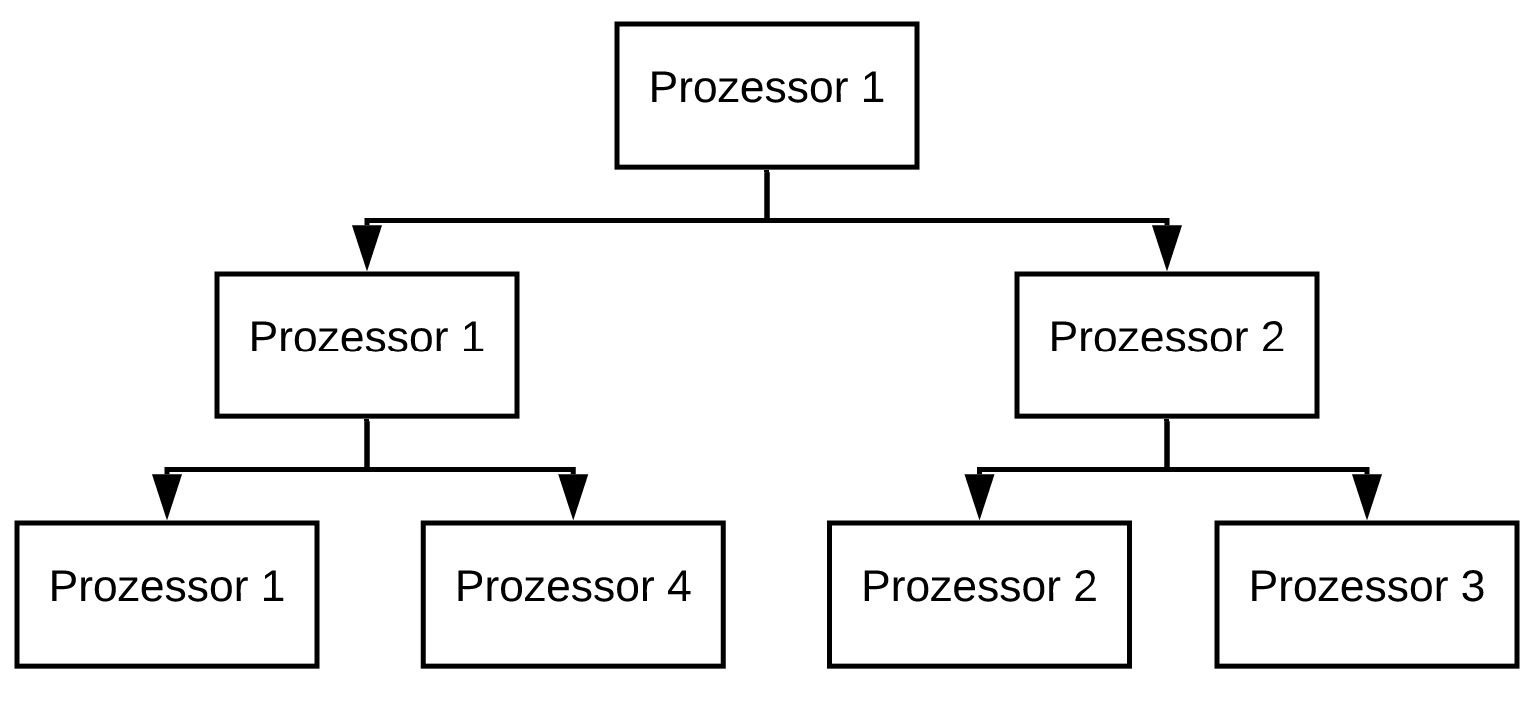
\includegraphics[width=\textwidth]{Images_Output/Parallel_Quicksort.png}
  \caption{Parallelized quicksort algorithm, retrived from \cite{parallelized_quicksort}}
  \label{fig:parallel_quicksort}
\end{figure}

\begin{figure}[H]
  \centering
  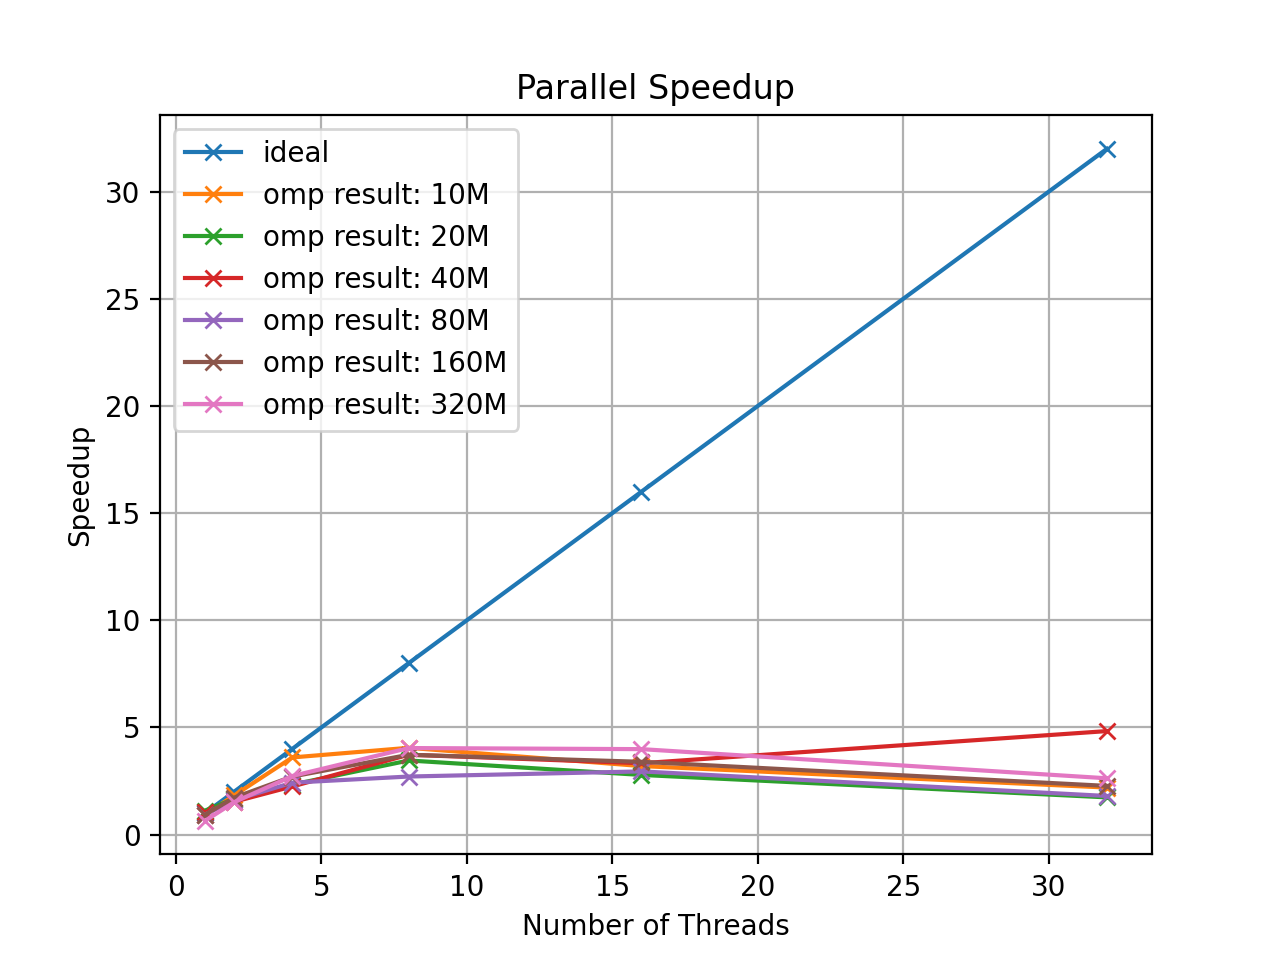
\includegraphics[width=\textwidth]{Images_Output/qicksort_tot_plot.png}
  \caption{Quicksort algorithm, retrived from \cite{parallelized_quicksort}}
  \label{fig:quicksort}
\end{figure}

\newpage
\section{Appendix}% Add to table of contents without numbering
In this section all results and the complete output data can be found.

\begin{figure}[H]
  \centering
  {\fontsize{8}{10}\selectfont
  \VerbatimInput{Images_Output/hist_output.txt}}
  \caption{Parallelized Code Snippet}
  \label{fig:slurm_euler_2}
\end{figure}

\begin{figure}[H]
  \centering
  {\fontsize{8}{10}\selectfont
  \VerbatimInput{Images_Output/output_mandel.txt}}
  \caption{Parallelized Code Snippet}
  \label{fig:slurm_euler_2}
\end{figure}

\begin{figure}[H]
  \centering
  {\fontsize{8}{10}\selectfont
  \VerbatimInput{Images_Output/output_recur.txt}}
  \caption{Parallelized Code Snippet}
  \label{fig:slurm_euler_2}
\end{figure}

\begin{figure}[H]
  \centering
  {\fontsize{8}{10}\selectfont
  \VerbatimInput{Images_Output/output_quicksort.txt}}
  \caption{Parallelized Code Snippet}
  \label{fig:slurm_euler_2}
\end{figure}


\newpage
% \section*{References}  % Use \section* to prevent section number
\addcontentsline{toc}{section}{References}  % Add to table of contents without numbering

\bibliographystyle{unsrt}
\bibliography{library}


\end{document}
